\chapter{Surface Heat Flux}

CFAST includes calculation of heat flux via convection, radiation, and conduction to compartment surfaces and targets. Heat transfer to the inside surface of compartment linings and the front and rear faces (as specified by the user) of targets consists of convection (through the use of empirical correlations) and radiation (calculated by the model using view factors for the fire, gas layers, and compartment surfaces). Heat conduction into a solid surface is calculated via a one-dimensional solution of the heat equation in cartesian or cylindrical coordinates.  The latter is particularly useful for predicting the thermal response of electrical cables.

For compartment linings, the ``outside'' surface is, by default, exposed to the exterior ambient temperature with convection and radiation calculated in a similar manner to the inside surface.  The ``outside'' boundary condition can also be specified as a constant temperature (i.e., the outside surface can be at ambient temperature) or can be connected to the ``outside'' surface of part or all of a second compartment.  For targets, the back surface is simply pointed in a direction opposite that of the front surface with convection and radiation calculated in a similar manner to the front surface. This chapter contains a variety of heat flux measurements, ranging from less than a kW/m$^2$ from very small gas burners  to more than 100~kW/m$^2$ in full-scale compartment fires.

\section{Heat Flux to  Compartment Ceiling, Wall, and Floor Surfaces}

In the NIST/NRC tests, heat flux gauges and thermocouples were positioned at various locations on the walls, floor, and ceiling of the fire compartments. The locations are given in Table~\ref{NIST_NRC_Wall_Coords}. The heat flux gauges were not water cooled; thus, they measured the {\em net} rather than the {\em gauge} heat flux. However, the net heat flux is a function of the temperature of the heat flux gauge itself, which is not something that is modeled. To better compare model and measurement, the measured net heat flux is converted into a gauge heat flux using the following formula:
\begin{equation}
\dot{q}''_{\subscript{gauge}} = \dot{q}''_{\subscript{net}} + \sigma \left( T^4_{\subscript{gauge}} - T^4_\infty \right) + h  \left( T_{\subscript{gauge}}-T_\infty \right) \quad \hbox{kW/m}^2
\end{equation}
where $\sigma=5.67 \times 10^{-11}$~kW/m$^2$/K$^4$ and $h=0.005$~kW/m$^2$/K.

Also, over the course of 15 experiments, numerous heat flux gauges failed, most often due to loss of contact with the wall or faulty thermocouples. All of the measurements from Test~13 and 16 were found to be flawed.

In the WTC tests, there were a variety of heat flux gauges installed in the test compartment. Most were within 2~m of the fire. Their locations and orientations are listed in Table~\ref{WTC_Gauges}. This section contains the measurements at the floor and ceiling.

\begin{table}[h!]
\caption{Heat flux gauge positions relative to the center of the fire pan in the WTC series.}
\begin{center}
\begin{tabular}{|l|c|c|c|c|l|}
\hline
Name    & $x$ (m)   & $y$ (m) & $z$ (m)   & Orientation  & Location  \\ \hline \hline
H2FU    & 0.64      & 0.63    & 3.30      &     $+z$     & Truss Support         \\ \hline
H2RU    & 0.64      & 0.51    & 3.30      &     $+z$     & Truss Support          \\ \hline
H2FD    & 0.64      & 0.30    & 3.15      &     $-z$     & Truss Support          \\ \hline
H2RD    & 0.64      & 0.42    & 3.15      &     $-z$     & Truss Support          \\ \hline
HCoHF   & -0.90     & 0.84    & 3.46      &     $+x$     & Column, facing fire          \\ \hline
HCoHW   & -0.97     & 0.92    & 3.27      &     $+y$     & Column, facing north          \\ \hline
HCoLF   & -0.90     & 0.84    & 0.92      &     $+x$     & Column, facing fire          \\ \hline
HCoLW   & -0.97     & 0.92    & 1.02      &     $+y$     & Column, facing north          \\ \hline
HF1     & 1.06      & 0.13    & 0.13      &     $+z$     & Floor          \\ \hline
HF2     & 1.56      & 0.10    & 0.13      &     $+z$     & Floor          \\ \hline
HCe1    & -0.45     & 0.35    & 3.82      &     $-z$     & Ceiling          \\ \hline
HCe2    &  0.05     & 0.35    & 3.82      &     $-z$     & Ceiling          \\ \hline
HCe3    &  0.80     & 0.35    & 3.82      &     $-z$     & Ceiling          \\ \hline
HCe4    &  2.56     & 0.35    & 3.82      &     $-z$     & Ceiling          \\ \hline
\end{tabular}
\end{center}
\label{WTC_Gauges}
\end{table}

Figure \ref{fig:Surface_Flux_Scatter} shows a comparison of predicted and measured values for total heat flux. Appendix B provides comparisons of heat flux and surface temperature on cable and surface targets.  The following trends are notable comparing CFAST predictions to experimental measurements.
\label{Target Heat Flux}

\begin{figure}
\begin{center}
\includegraphics[width=4in]{FIGURES/ScatterPlots/Surface_Heat_Flux}
\end{center}
\caption{Comparisons of Measured and Predicted Compartment Surface Temperature} \label{fig:Surface_Flux_Scatter}
\end{figure}

\begin{itemize}
\item Overall, surface heat flux averages within \Surfacefluxavg ~\% of experimental values.  Like surface temperature, there is considerable spread in the data
\item Typically, CFAST over-predicts the far-field fluxes and temperatures and under-predicts the near-field measurements.  This is understandable, given that any two-zone model predicts an average representative value of gas temperature in the upper and lower regions of a compartment so that convective heat transfer is fairly uniform to ceiling/upper wall and lower wall/floor surfaces.  Thus, the values predicted by CFAST should roughly be an average of values near the fire and those farther away.
\item However, differences for the ceiling and (particularly) floor heat fluxes are higher, with a more pronounced difference between the near-field and far-field comparisons.  In addition to the limitations of the two-zone assumption, calculations of the flux to ceiling and floor surfaces are further confounded by the simple point-source calculation of radiation exchange in CFAST for the fire source.  In CFAST, the fire is assumed to be a point source of energy located at mid-height in the fire rather than a three-dimensional flame surface radiating to surroundings.  With the fire typically at the floor surface, this makes the calculation of flux to the floor surface inherently less accurate than for other surfaces.
\end{itemize}

\section{Heat Flux to Targets}

In the NIST/NRC tests, cables in various types (power and control), and configurations (horizontal, vertical, in trays or free-hanging), were installed in the test compartment. For each of the four cable targets considered, measurements of the radiative and total heat flux were made with gauges positioned near the cables themselves.  In the WTC tests, There were a variety of heat flux gauges installed in the test compartment. Most were within 2~m of the fire. Their locations and orientations are listed in Table~\ref{WTC_Gauges}. Figure \ref{fig:Target_Flux_Scatter} shows a comparison of predicted and measured values for total heat flux. Appendix B provides comparisons of heat flux and surface temperature on cable and surface targets.  The following trends are notable comparing CFAST predictions to experimental measurements.
\label{Surface Heat Flux}
\label{Wall Heat Flux}
\label{Ceiling Heat Flux}
\label{Floor Heat Flux}

\begin{figure}
\begin{center}
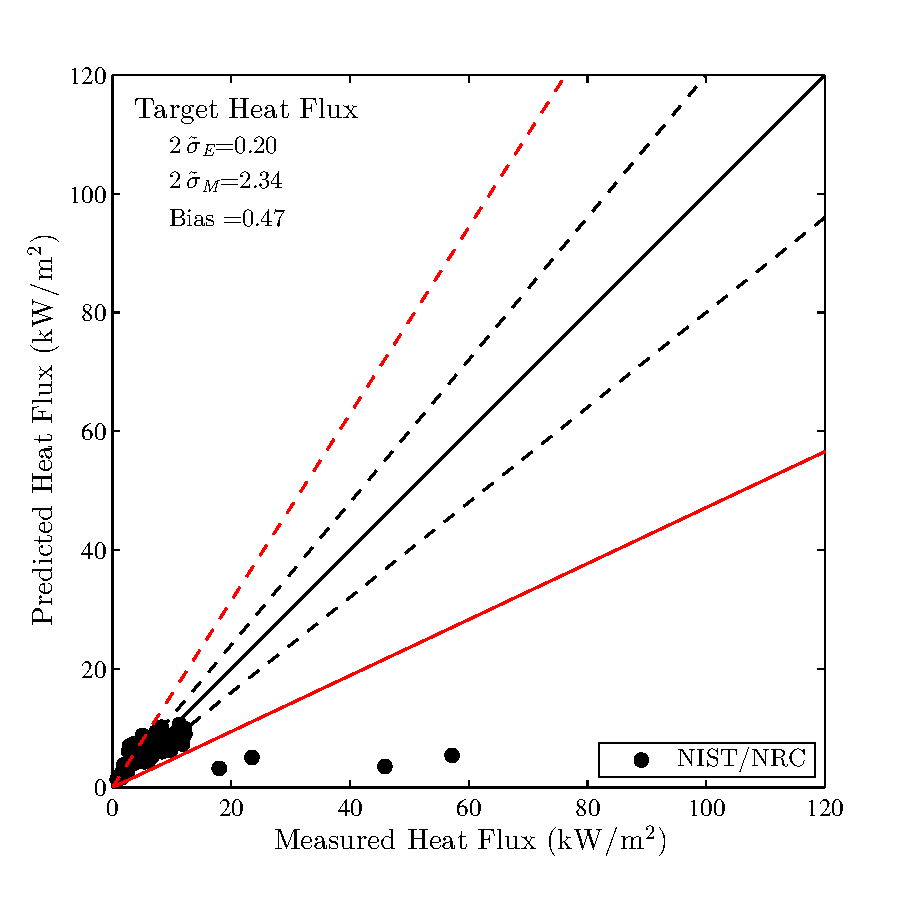
\includegraphics[width=4in]{FIGURES/ScatterPlots/Target_Heat_Flux}
\end{center}
\caption{Comparisons of Measured and Predicted Heat Flux to Targets} \label{fig:Target_Flux_Scatter}
\end{figure}

\begin{itemize}
\item Heat flux to targets average within \Targfluxavg ~\% of experimental values. This high value is largely driven by four data points in the NIST/NRC tests that are significantly under-predicted by the model.  Without these data points, the uncertainty is significantly lower.
\item The higher value for target heat flux is also due to the way CFAST calculates flux to targets.  The calculation of heat flux to a target in CFAST is done separately for the front face and rear face of the target.  For target completely within a compartment, these two values are typically similar.  For target on a compartment surface, the rear surface is assumed to radiate to ambient conditions.  Thus, considering only the front face in the comparison should lead to a significant indicated overprediction of the heat flux. The predicted surface temperature is predicted far closer to experimental conditions that the surface heat flux indicating the actual heat flux is likely better than indicated by this front-face only comparison.
\item  In addition, prediction of heat flux to targets is even more dependent on local conditions than surface temperature and heat flux.  Like any two-zone model, CFAST predicts an average representative value of gas temperature in the upper and lower regions of a compartment.  In addition, CFAST does not directly predict plume temperature or its effects on targets that may be within a fire plume.  Thus, CFAST can be expected to under-predict values near a fire source, and over-predict values for targets remote from a fire.
\end{itemize}
